\documentclass{beamer}


\usepackage{graphics}
\usepackage{graphicx}
\usepackage{hyperref}
\usepackage[latin1]{inputenc}

\usepackage{listings}
\lstset{showstringspaces=false,frame=trBL,frameround=tttt,tabsize=8,basicstyle=\tiny,breaklines=true,breakatwhitespace=true}
\lstdefinestyle{bash}{language=bash}
\lstdefinestyle{Perl}{language=Perl}
\lstdefinestyle{C++}{language=C++}
\lstdefinestyle{DTD}{language=XML}
\lstdefinestyle{XML}{language=XML,usekeywordsintag=false,markfirstintag=true}
\newcommand{\includecode}[2]{\lstinputlisting[style=#1]{#2}}
%\lstnewenvironment{code}{}{}
\lstnewenvironment{code_bash}{\lstset{style=bash}}{}
\lstnewenvironment{code_perl}{\lstset{style=Perl}}{}
\lstnewenvironment{code_cpp}{\lstset{style=C++}}{}
\lstnewenvironment{code_dtd}{\lstset{style=DTD}}{}
\lstnewenvironment{code_xml}{\lstset{style=XML}}{}

\newcommand{\textcode}[1]{{\small {\tt #1}}}

% ---- format de page A4
% 	\setlength{\textwidth }{16cm}	% largeur de ligne
% 	\setlength{\textheight}{23cm}   % hauteur du texte
	\setlength{\oddsidemargin}{-17mm} % marge pages impaires
	\setlength{\evensidemargin}{-17mm}% marge pages paires
% 	\setlength{\topmargin}{0cm} 	
% 	\setlength{\headheight}{14pt} 
% 	\setlength{\headsep}{0.5cm} 

\title[Scen graph equations]{From scene graph to equations}
\author[Faure]{%
  Fran�ois~Faure\inst{1} }
\institute[Univ. Grenoble]{
  \inst{1}%
  Grenoble Universities\\
  INRIA - Evasion
  }
\date[September 2007]{September 2007}
\subject{Computational Sciences}

\newcommand{\svec}[1]{\ensuremath{\left( \begin{array}{c} {#1}_1 \\ {#1}_2 \end{array} \right)}}
\newcommand{\smatm}{\ensuremath{
\left(\begin{array}{cc}
 M_1 & \\
& M_2
\end{array}
\right)
}}
\newcommand{\smatc}{\ensuremath{
\left(\begin{array}{cc}
 C_1 & \\
& C_2
\end{array}
\right)
}}
\newcommand{\smatk}{\ensuremath{
\left(\begin{array}{cc}
 K_{11} & K_{12}\\
K_{21} & K_{22}
\end{array}
\right)
}}

\begin{document}

  \frame
  {
    \titlepage
  }

\begin{frame}
 \frametitle{A physical body}
\begin{center}
 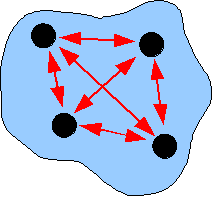
\includegraphics[width=0.35\linewidth]{body.png}
\end{center}
State vectors: $x$, $v$, $f$, $a$, $aux$, ...\\
Influenced by:
\begin{itemize}
 \item Force $f(x,v)$ and stiffness $K = \frac{df}{dx}$
 \item Mass $M$
 \item Constraints $c(x)$, $C$ 
\end{itemize}
\end{frame}


\begin{frame}
 \frametitle{Two bodies interacting}
\begin{columns}
\column{0.6\linewidth}
\begin{itemize}
 \item Body 1: 
\begin{itemize}
 \item $x_1$, $v_1$, $f_1$
 \item $f_1(x_1,v_1)$, $K_{11}(x_1)$
 \item $M_1$
 \item $c_1(x)$, $C_1$
\end{itemize}
 \item Interaction 1-2: 
\begin{itemize}
 \item[1$\rightarrow$2] $f_{12}(x_1,v_1,x_2,v_2)$, $K_{12}(x_1,v_1,x_2,v_2)$
 \item[2$\rightarrow$1] $f_{21}(x_1,v_1,x_2,v_2)$, $K_{21}(x_1,v_1,x_2,v_2)$
\end{itemize}
 \item Body 2 %$x_2$, $v_2$, $f_2(x_2,v_2)$, $K_{22}(x_2)$, $M_2$
\end{itemize}
\column{0.39\linewidth}
\begin{center}
 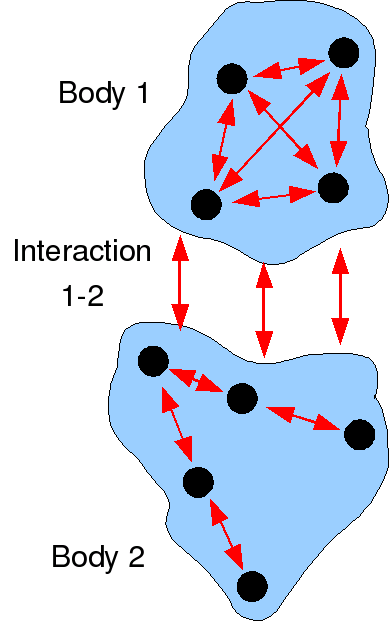
\includegraphics[width=\linewidth]{bodies.png}
\end{center}
 
\end{columns}
\end{frame}


\begin{frame}[fragile]
 \frametitle{Implicit Euler}
\begin{columns}
\column{0.7\linewidth}
Solve $C(M + h^2K)C\Delta v = hC(f+hKv)$
\begin{itemize}
 \item $C$ models constraints as filters
\end{itemize}

Apply conjugate gradient solution
\begin{itemize}
 \item Does not address the entries of the matrix
 \item Performs only matrix-vector products and vector products
 \item Products can be performed blockwise, in any order
\end{itemize}

\column{0.29\linewidth}
\begin{center}
 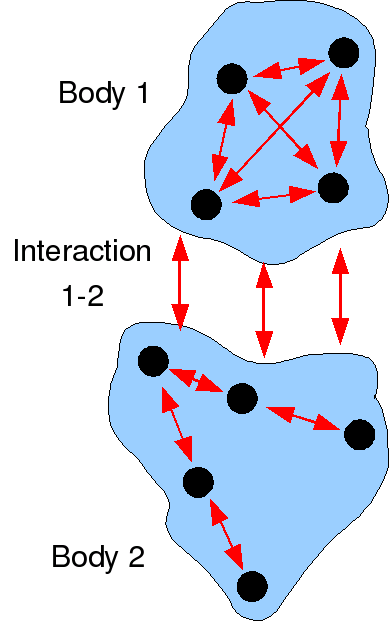
\includegraphics[width=\linewidth]{bodies.png}
\end{center}
\end{columns}
\end{frame}



\begin{frame}
 \frametitle{State vectors}
\begin{columns}
\column{0.7\linewidth}
\begin{itemize}
 \item positions x=\svec{x}
 \item velocities v=\svec{v}
 \item auxiliary vectors a=\svec{a}, aux=\svec{aux}...
 \item force f=\svec{f}=$\left(\begin{array}{c}
 f_1(x_1,v_1) + f_{12}(x_1,v_1,x_2,v_2) \\
 f_2(x_2,v_2) + f_{21}(x_1,v_1,x_2,v_2)
\end{array}\right)$

\end{itemize}
\column{0.29\linewidth}
\begin{center}
 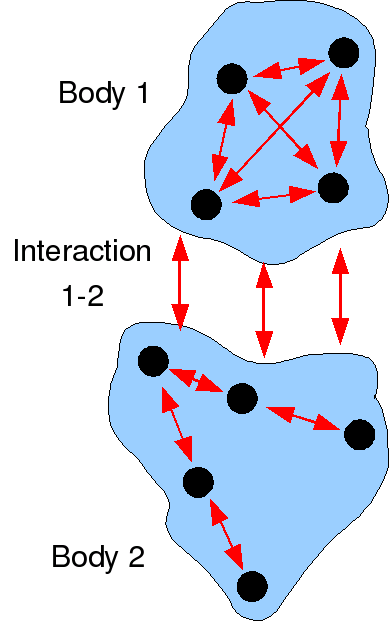
\includegraphics[width=\linewidth]{bodies.png}
\end{center}
\end{columns}
\end{frame}



\begin{frame}
 \frametitle{Vector operations}
\begin{columns}
\column{0.7\linewidth}
\begin{itemize}
 \item  Sums are computed in parallel: $$x+ay = \left(\begin{array}{c}
 x_1 + a y_1\\ 
x_2 + a y_2
\end{array}
\right)
$$
\item Dot products require to sum over all objects: $$x^Ty = x_1^Ty_1 + x_2^Ty_2$$
\item State vectors can be stored and processed in parallel in each body
\item They can even have different types in different bodies, \textit{e.g.} particles and a rigid body
\end{itemize}
\column{0.29\linewidth}
\begin{center}
 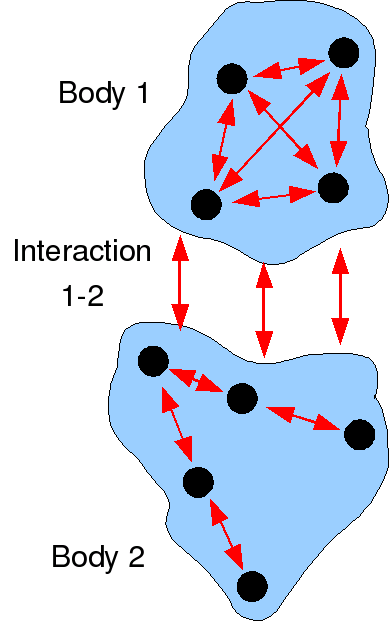
\includegraphics[width=\linewidth]{bodies.png}
\end{center}
\end{columns}
\end{frame}



\begin{frame}
 \frametitle{System matrices}
\begin{columns}
\column{0.8\linewidth}
Block structure: 
\begin{itemize}
 \item $M=\smatm$ Mass matrix, block-diagonal 
 \item $K=\smatk$ Stiffness matrix, generally sparse
 \item $C=\smatc$ Filter matrix, block-diagonal
\end{itemize}

\column{0.19\linewidth}
\begin{center}
 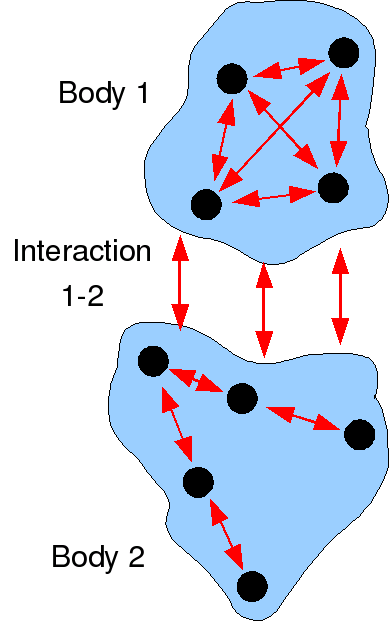
\includegraphics[width=\linewidth]{bodies.png}
\end{center}
\end{columns}

Conjugate gradient solution:
\begin{itemize}
 \item We do not need to address the entries of the matrices
 \item We need to compute their products with vectors
\end{itemize}
\end{frame}


\begin{frame}
 \frametitle{Matrix-vector product}
% \begin{columns}
% \column{0.8\linewidth}
\begin{center}
 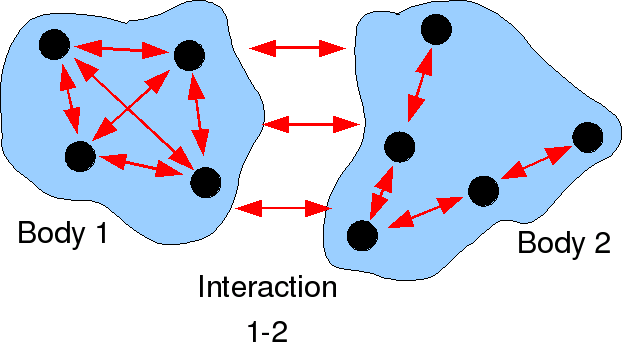
\includegraphics[width=0.4\linewidth]{bodies-horiz.png}
\end{center}
\begin{itemize}
 \item Without constraints:
$$(M+h^2K)y = \left( \begin{array}{c}
 M_{11}y_1 + h^ 2K_{11}y_1 + h^2K_{12}y_2 \\
 M_{22}y_2 + h^ 2K_{22}y_2 + h^2K_{21}y_1 
\end{array}
\right)
$$
 \item With constraints:
$$C(M+h^2K)Cy = \left( \begin{array}{c}
C_1M_{11}C_1y_1 + h^ 2C_1K_{11}C_1y_1 + h^2C_1K_{12}C_2y_2 \\
 C_2M_{22}C_2y_2 + h^ 2C_2K_{22}C_2y_2 + h^2C_2K_{21}C_1y_1 
\end{array}
\right)
$$
\end{itemize}
% \column{0.19\linewidth}
% \end{columns}
\end{frame}


% \begin{frame}
%  \frametitle{State vectors}
% \begin{columns}
% \column{0.7\linewidth}
% \begin{itemize}
%  \item 
% \end{itemize}
% \column{0.29\linewidth}
% \begin{center}
%  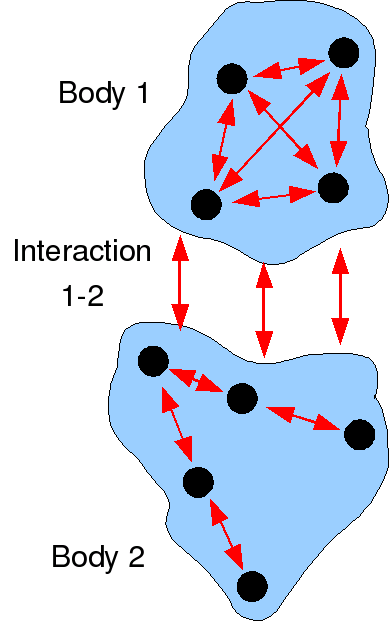
\includegraphics[width=\linewidth]{bodies.png}
% \end{center}
% \end{columns}
% \end{frame}



% \begin{frame}
%  \frametitle{Conjugate gradient solution}
% \begin{itemize}
%  \item Does not addess the entries of the matrix
%  \item Performs only matrix-vector products and vector products
%  \item Products can be performed blockwise, in any order
% \end{itemize}
% Without constraints:
% $(M+h^2K)y = \left( \begin{array}{c}
%  M_{11}y_1 + h^ 2K_{11}y_1 + h^2K_{12}y_2 \\
%  M_{22}y_2 + h^ 2K_{22}y_2 + h^2K_{21}y_1 
% \end{array}
% \right)
% $
% With constraints:
% $C(M+h^2K)Cy = \left( \begin{array}{c}
% C_1M_{11}C_1y_1 + h^ 2C_1K_{11}C_1y_1 + h^2C_2K_{12}C_2y_2 \\
%  C_2M_{22}C_2y_2 + h^ 2C_2K_{22}C_2y_2 + h^2C_2K_{21}C_1y_1 
% \end{array}
% \right)
% $
% \end{frame}

\begin{frame}
 \frametitle{Scene structure and elementary operations}
System of bodies
\begin{itemize}
 \item Body 1
\begin{itemize}
 \item State vectors x, v, f, aux1, ...
 \item Mass: $M_1*, \;\;M_1^{-1}*$
 \item Force(s): $+=f_1(x_1,v_1), \;\; +=K_1*$
 \item Filter(s): $c(x_1),\;\; C_1*$
\end{itemize}
 \item Body 2
 \item Interaction 1-2
\begin{itemize}
 \item $+=f_{12}(),\;\;+=f_{21}(),\;\;+=K_{12}*, \;\; +=K_{21}*$
\end{itemize}

\end{itemize}

\end{frame}



\begin{frame}
 \frametitle{Right-hand term of the implicit integration}
\begin{itemize}
 \item vector to compute:$$b=hC(f(x,v)+hK(x)v)$$
 \item operations: \begin{tabular}{|l|l|}
 & propagateState(x,v) \\
$b_i = 0$ & b.clear() \\
$b_i += K_{ii} v_i$ & AccumulateDForceAction(b,v) \\
$b_i += K_{ij} v_j$ & \\
$b_i *= h $& v\_teq(b,h) \\
$b_i += f_i(x_i,v_i)$ & AccumulateForceAction(b)\\ 
$b_i *= h $ & v\_teq(b,h) \\
$b_i = C_i b_i$ & ApplyConstraintsAction(b)
\end{tabular}
\item PropagateStateAction updates the force and stiffness operators    
\end{itemize}
\end{frame}

\begin{frame}
 \frametitle{Computation of a matrix-vector product}
\begin{itemize}
 \item In each body i: $$f_i = (C(M+h^2K)Cy)_i = C_i(M_{ii}+h^2K_{ii})C_iy_i + C_ih^2\sum_{j\neq i}K_{ij}C_jy_j$$
\item Operations:\begin{tabular}{|l|l|}
$f_i = 0$ & f.clear() \\
$y_i = C_i y_i$ & ApplyConstraintsAction(y) \\
$f_i += M_i y_i$ & ApplyMassAction(f,y) \\
$f_i += K_{ii} y_i$ & AccumulateDForceAction(f,y) \\
$f_i += K_{ij} y_j$ &\\ 
$f_i = C_i f_i$ & ApplyConstraintsAction(f)
\end{tabular}
\end{itemize}
\end{frame}


\begin{frame}
 \frametitle{Mapped points}
example: points attached to a rigid body
\begin{columns}
 \column{0.6\linewidth}
position: $p = o + R(op)$
velocity: $v = v_o + po \times \Omega$
$$
 \left(
\begin{array}{c}
 \Omega \\ v_p
\end{array}
\right)
=
 \left(
\begin{array}{c}
 \Omega \\ v_o + po \times \Omega
\end{array}
\right)
=
 \left(
\begin{array}{cc}
 I & po \times\\
 & I
\end{array}
\right)
 \left(
\begin{array}{c}
 \Omega \\ v_o + po \times \Omega
\end{array}
\right)
= Jv
$$

force in p: 
$\left( \begin{array}{c}
 f_p \\ \tau_p 
\end{array} \right) 
=
\left( \begin{array}{c}
 f_o = f_p \\ \tau_o = \tau_p + op \times f_o 
\end{array} \right) 
$
and 
$$
 \left(
\begin{array}{c}
 f_o \\ \tau_o
\end{array}
\right)
=
 \left(
\begin{array}{c}
 f_p = f_o \\ 
\tau_p = \tau_o + op \times f_o
\end{array}
\right)
=
 \left(
\begin{array}{cc}
 I & \\
 op\times & I
\end{array}
\right)
 \left(
\begin{array}{c}
 \Omega \\ v_o + po \times \Omega
\end{array}
\right)
= J^Tf
$$

\column{0.39\linewidth}
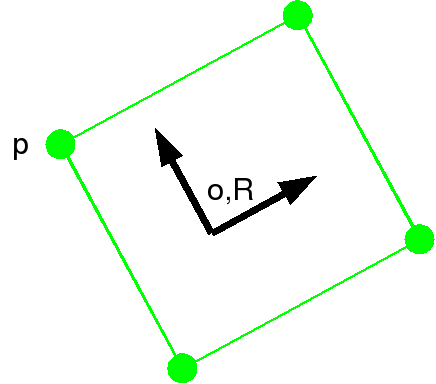
\includegraphics[width=\linewidth]{map-x.png}
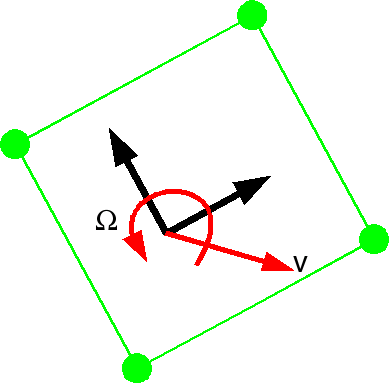
\includegraphics[width=\linewidth]{map-v.png}
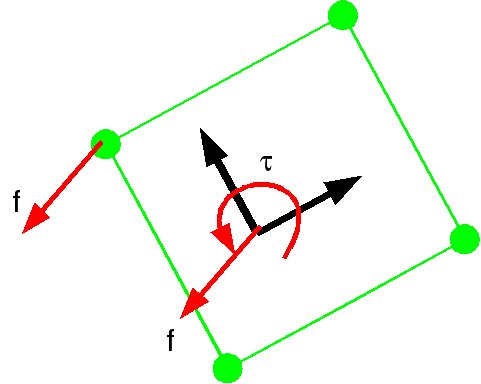
\includegraphics[width=\linewidth]{map-f.png}
\end{columns}

\end{frame}



\begin{frame}
 \frametitle{Mapping child forces to the parent DOF}
Given $v_c = J v_p$ and force $f_c$ applied to the child, the equivalent parent force is: 
$$ f_p = J^T f_c$$
Proof:
To be equivalent, $f_c$ and $f_p$ must have the sma virtual power:
\begin{eqnarray*}
 f_p^Tv_p &=& f_c^Tv_c \mbox{for any} v_p \\
 &=& f_c^TJv_p \mbox{for any} v_p \\
f_p^T &=& f_c^TJ  \\
f_p &=& J^Tf_c
\end{eqnarray*}
\end{frame}


\begin{frame}
 \frametitle{}
\end{frame}



\end{document}
